% % ***********************************************************
% ******************* PHYSICS HEADER ************************
% ***********************************************************
% Version 2

\usepackage{amsmath} % AMS Math Package
\usepackage{amsthm} % Theorem Formatting
\usepackage{amssymb}	% Math symbols such as \mathbb
\usepackage{graphicx} % Allows for eps images
\usepackage{multicol} % Allows for multiple columns
\usepackage[dvips,showframe,letterpaper,margin=1.0in,left=1.5in]{geometry}
% tim included
\usepackage[pdftex,bookmarks=true]{hyperref}

\usepackage{cancel}
\usepackage{siunitx}
 % Sets margins and page size
\pagestyle{plain} % Removes page numbers
\makeatletter % Need for anything that contains an @ command 
\renewcommand{\maketitle} % Redefine maketitle to conserve space
{ \begingroup \vskip 10pt \begin{center} \large {\bf \@title}
	\vskip 10pt \large \@author \hskip 20pt \@date \end{center}
  \vskip 10pt \endgroup \setcounter{footnote}{0} }
\makeatother % End of region containing @ commands
\renewcommand{\labelenumi}{(\alph{enumi})} % Use letters for enumerate
% \DeclareMathOperator{\Sample}{Sample}
\let\vaccent=\v % rename builtin command \v{} to \vaccent{}
\renewcommand{\v}[1]{\ensuremath{\mathbf{#1}}} % for vectors
\newcommand{\gv}[1]{\ensuremath{\mbox{\boldmath$ #1 $}}} 
% for vectors of Greek letters
\newcommand{\uv}[1]{\ensuremath{\mathbf{\hat{#1}}}} % for unit vector
\newcommand{\abs}[1]{\left| #1 \right|} % for absolute value
\newcommand{\avg}[1]{\left< #1 \right>} % for average
\let\underdot=\d % rename builtin command \d{} to \underdot{}
\renewcommand{\d}[2]{\frac{d #1}{d #2}} % for derivatives
\newcommand{\dd}[2]{\frac{d^2 #1}{d #2^2}} % for double derivatives
\newcommand{\pd}[2]{\frac{\partial #1}{\partial #2}} 
% for partial derivatives
\newcommand{\pdd}[2]{\frac{\partial^2 #1}{\partial #2^2}} 
% for double partial derivatives
\newcommand{\pdc}[3]{\left( \frac{\partial #1}{\partial #2}
 \right)_{#3}} % for thermodynamic partial derivatives
\newcommand{\ket}[1]{\left| #1 \right>} % for Dirac bras
\newcommand{\bra}[1]{\left< #1 \right|} % for Dirac kets
\newcommand{\braket}[2]{\left< #1 \vphantom{#2} \right|
 \left. #2 \vphantom{#1} \right>} % for Dirac brackets
\newcommand{\matrixel}[3]{\left< #1 \vphantom{#2#3} \right|
 #2 \left| #3 \vphantom{#1#2} \right>} % for Dirac matrix elements
\newcommand{\grad}[1]{\gv{\nabla} #1} % for gradient
\let\divsymb=\div % rename builtin command \div to \divsymb
\renewcommand{\div}[1]{\gv{\nabla} \cdot #1} % for divergence
\newcommand{\curl}[1]{\gv{\nabla} \times #1} % for curl
\let\baraccent=\= % rename builtin command \= to \baraccent
\renewcommand{\=}[1]{\stackrel{#1}{=}} % for putting numbers above =
\newtheorem{prop}{Proposition}
\newtheorem{thm}{Theorem}[section]
\newtheorem{lem}[thm]{Lemma}
\theoremstyle{definition}
\newtheorem{dfn}{Definition}
\theoremstyle{remark}
\newtheorem*{rmk}{Remark}

% ***********************************************************
% ********************** END HEADER *************************
% *********************************************************** 
% \newcommand{\sigdot}[1]{ \gv{\sigma} \hspace{-2pt} \cdot \hspace{-2pt} \v{#1} \,}
% \newcommand{\sigdotg}[1]{ \gv{\sigma} \hspace{-2pt} \cdot \hspace{-2pt} \gv{#1} \,}
% \newcommand{\dotprod}[2]{ \v{#1} \hspace{-2pt} \cdot \hspace{-2pt} \v{#2} \,}

%\newcommand{\beqa}{\begin{eqnarray*} }
%\newcommand{\eeqa}{\end{eqnarray*} }

% \newcommand{\diracdelta}[1]{ \delta^{(3)}(#1) }
% \newcommand{\omin}[1]{ \W_{#1}(p) }
% \newcommand{\omout}[1]{ \W^*_{#1}(p') }
% 
% \newcommand{\E}[1]{ \sqrt{ m^2 + \v{#1}^2 } }
% \newcommand{\E}[1]{ E_{#1} }
% \newcommand{\A}{a}
% \newcommand{\Adag}{a'}
% \newcommand{\qp}{q^{(+)}{}}
% \newcommand{\qm}{q^{(-)}{}}
% 
% \newcommand{\smalldot}{\cdot}
% 
% \newcommand{\gradE}{\grad}
% 
% 
% \newcommand{\snote}[1]{ \small {\bf Sign note:} \emph{ #1} \normalsize }
\chapter{Diagrammatic approach to spin-one particles}

%TODO rename this
\section{Introduction}
In the previous section, a nonrelativistic Hamiltonian was derived from a relativistic Lagrangian of a charged spin one particle, by solving the equations of motion for the energies of the fields.  As in the case of a spin one-half particle, there is an alternate approach.  The most general NRQED Lagrangian for a spin one particle interacting with an electromagnetic field can be written down.  Then, by considering the same physical processes in the NRQED theory and the initial relativistic spin one theory, the coefficients in the NRQED Lagrangian may be fixed.

As for spin one-half, the most appropriate physical processes to consider are scattering off an external magnetic field and Compton scattering.  (The latter is not strictly necessary, but is a check of the consistency of the calculation.)

First the NRQED Lagrangian for a spin one particle will be developed.  Then, the scattering processes will be calculated from this Lagrangian.  Next the same processes will be calculated in the relativistic theory, and a connection between the relativistic polarisations and nonrelativistic spinors established.  Finally the two calculations will be compared, and thus the NRQED Lagrangian determined.  

\section{Nonrelativistic Lagrangian for spin one}

For spin half, the NRQED Lagrangian \eqref{eq:Sh:nrL-2f} has been constructed.  All of the terms that exist in that Lagrangian can occur in the spin one Lagrangian as well.  So what must be established is what type of new terms arise in the higher spin theory.

All the ``building blocks'' used in constructing the spin half theory may be used: the fields $\v{E}$ and $\v{B}$, the gauge invariant derivative $\v{D}$, and the spin operator $\v{S}$.  In moving from spin half to spin one, the only new terms allowed are those that are quadratic in $S$.  In the spin half theory, the fields had two components, and so together with the identity, the set $S_i$ completely spanned the space of Hermitian spin operators.  In spin one the nonrelativistic fields have three components, and so the basis for spin operators is larger.

To ensure that new terms introduced are completely independent of those specific to spin half, combinations of $S$ matrices which vanish for spin half should be considered.  The appropriate combination is the symmetric, traceless structure $\Sb_{ij} \equiv S_i S_j + S_j S_i - (2/3) S^2 \delta_{ij}$, which for spin one is $S_i S_j + S_j S_i - (4/3) \delta_{ij}$.

So, any new term will be some combination of $\Sb_{ij}$ and $E$, $B$, and $D$.  $\Sb_{ij} B_i D_j$ and $\Sb_{ij} B_i E_j$ are banned by parity, and terms quadratic in $B$ are not considered.  Terms quadratic in $E$ are also too high order.  And $\Sb_{ij} D_i D_j$ is not allowed because it would spoil the structure of the kinetic term.

So the only new term that arises involves $\Sb_{ij}$, $E$, and $D$.  The Hermitian combination of these of the proper dimension is
\beq	
	\frac{e}{8m^2} \ \Sb_{ij} ( E_i D_j - D_j E_i) = \frac{e \Sb_{ij} \partial_i E_j  }{8m^2} 
\eeq

This structure is related to the quadrupole moment, so label the coefficient $c_Q$.  Then, the complete spin one Lagrangian will be
\scriptsize \label{eq:S1:Lnr}
\beqa
	\mathcal{L}_{NRQED} &=& \Psi^\dagger \{ i(\partial_0 + ieA_0) + \frac{\v{D}^2}{2m} + \frac{\v{D}^4}{8m^3} 
		+ c_F e \frac{\v{S} \smalldot \v{B}} {2m}   	
		+ c_D \frac{ e(\v{D} \smalldot \v{E} - \v{E} \smalldot \v{D} ) }{8m^2}	
		+ c_Q \frac{e \Sb_{ij} (D_i E_j - E_i D_j) }{8m^2}	
	\\&&	+ c_S \frac{ ie \v{S} \smalldot ( \v{D} \times \v{E} - \v{E} \times \v{D} )}{8m^2}
		+ c_{W_1} \frac{ e [ \v{D}^2 (\v{S} \smalldot \v{B} ) + (\v{S} \smalldot \v{B} ) \v{D}^2] }{8m^3}	
		- c_{W_2} \frac{ e D^i (\v{S} \smalldot \v{B} ) D^i }{4m^3}
		+ c_{p'p} \frac{ e [ (\v{S} \smalldot \v{D}) (\v{B} \smalldot \v{D}) + (\v{B} \smalldot \v{D})(\v{S} \smalldot \v{D}) }{8m^3} \} \Psi
\eeqa
\normalsize



%NOTE we use D = \partial - ieA
\subsection{Scattering off external field in NRQED}
With the Lagrangian in hand, the amplitude for the charged particle scattering off an external field can be calculated.  At the tree level (which is the only level contributing to the final calculation) the process involves just a single photon.  So consider those terms in the NRQED Lagrangian which contain one power of the external field.  


This calculation is largely the same as that for spin one-half, with the only change being the addition of the quadrupole term.  Augmented by this term, the Lagrangian \eqref{eq:Sh:nrL-2f} becomes 
\small
\beqa
\mathcal{L}_A &=& \Psi^\dagger (  -eA_0- ie  \frac{ \{\nabla_i, A_i \} }{2m} -ie \frac{ \{\grad^2, \{\nabla_i, A_i \}  \} }{8m^3} 
		+ c_F e \frac{\v{S} \smalldot \v{B}} {2m}   	
		+ c_D \frac{ e(\v{\grad} \smalldot \v{E} - \v{E} \smalldot \v{\grad} ) }{8m^2}	
		+ c_Q \frac{e Q_{ij} (\nabla_i E_j - E_i \nabla_j) }{8m^2}	
	\\&&	+ c^{1}_S \frac{ ie \v{S} \smalldot ( \v{\grad} \times \v{E} - \v{E} \times \v{\grad} )}{8m^2}
		+ c_{W_1} \frac{ e [ \v{\grad}^2 (\v{S} \smalldot \v{B} ) + (\v{S} \smalldot \v{B} ) \v{\grad}^2] }{8m^3}	
		- c_{W_2} \frac{ e \nabla^i (\v{S} \smalldot \v{B} ) \nabla^i }{4m^3}
		+ c_{p'p} \frac{ e [ (\v{S} \smalldot \v{\grad}) (\v{B} \smalldot \v{\grad}) + (\v{B} \smalldot \v{\grad})(\v{S} \smalldot \v{\grad}) }{8m^3} \big )\Psi
\eeqa
\normalsize


The process under consideration is this: scattering off an external field, with incoming momentum $\v{p}$, outgoing $\v{p'}$, and $\v{q} = \v{p'} - \v{p}$.  There is one diagram associated with each term above, but the total amplitude is just going to be the sum of all these one-photon vertices.  These of course can just be read off directly from the Lagrangian: replace the fields $\Psi$ with the spinors $\phi$, and any operator $\grad$ acting will become $i\v{p}$ if it acts on the right, $i\v{p'}$ if it is to the left.

Some expressions involving $\grad$ and $\v{E}$ can be simplified.  Because $Q_{ij}$ is symmetric:
\[
	 Q_{ij} (\nabla_i E_j - E_i \nabla_j ) = Q_{ij} [\nabla_i, E_j] = Q_{ij} (\partial_i E_j)
\]
And because $E_i = -\partial_i \Phi$
\[
	\v{\grad} \times \v{E} - \v{E} \times \v{\grad} =  - 2 \v{E} \times \v{\grad}
\]
And also use that
\[
\v{\grad} \smalldot \v{E} - \v{E} \smalldot \v{\grad} = (\partial_i E_i)
\]
Now the scattering amplitude for scattering off the external field can be written down.  Before any assumptions about the particular process are made, it is:
\beqa
	iM &=&
		ie\phi^\dagger \Bigg( - A_0 +    \frac{ \v{A} \cdot (\v{p} + \v{p'}) }{2m} 
		- \frac{  \v{A} \cdot (\v{p} + \v{p'}) \v{p}^2 + \v{p'}^2 \v{A} \cdot (\v{p} + \v{p'}) }{8m^3} 
	\\&&	+ c_F  \frac{\v{S} \smalldot \v{B}} {2m}   	
		+ c_D \frac{ ( \partial_i E_i ) }{8m^2}	
		+ c_Q \frac{Q_{ij}  ( \partial_i E_j ) }{8m^2}	
		+ c^{1}_S \frac{  \v{E} \times \v{p} }{4m^2}
	\\&&	- c_{W_1}  \frac{  (\v{S} \smalldot \v{B} ) (\v{p}^2 + \v{p'}^2)  }{8m^3}
		+ c_{W_2} \frac{  (\v{S} \smalldot \v{B} ) (\v{p} \cdot \v{p'}) }{4m^3}
		-  c_{p'p} \frac{  (\v{S} \smalldot \v{p'}) (\v{B} \smalldot \v{p}) + (\v{B} \smalldot \v{p'}) (\v{S} \smalldot \v{p}) }{8m^3} \Bigg )\phi
\eeqa

The above can be simplified somewhat.  The gauge can be chosen such that $\nabla_i A_i = 0$.  If elastic scattering is specified then kinematics dictate that $\v{p'}^2 = \v{p}^2$.   Finally, if $\v{B}$ is constant, the $c_W$ terms become indistinguishable, since $[ \nabla_i, B_j] = 0$.    (It is only this last assumption that costs us any information.)  Then the scattering amplitude, as calculated from $\mathcal{L}_{NRQED}$, is:

\beqa
	iM &=&
		ie\phi^\dagger \Bigg(  -A_0 +  \frac{ \v{A} \cdot \v{p} }{m} - \frac{  (\v{A} \cdot \v{p}) \v{p}^2   }{2m^3} 
		+ c_F  \frac{\v{S} \smalldot \v{B}} {2m}   	
		+ c_D \frac{ ( \partial_i E_i ) }{8m^2}	
		+ c_Q \frac{ Q_{ij} ( \partial_i E_j ) }{8m^2}	
	\\&&	+ c^{1}_S \frac{  \v{E} \times \v{p} }{4m^2}
		- (c_{W_1} -c_{W_2}) \frac{   (\v{S} \smalldot \v{B} ) \v{p}^2  }{4m^3}	
		-  c_{p'p} \frac{   (\v{S} \smalldot \v{p}) (\v{B} \smalldot \v{p})  }{4m^3} \Bigg )\phi
\eeqa

Calculating the scattering amplitude for the same process in the relativistic theory will fix the unknown coefficients.  Then the NRQED Lagrangian can be used in other calculations, such as for the bound $g$-factor. 

%%%%%%%%%%%%%%%%%%%%%%%%%%%%%
% TWO PHOTON
%%%%%%%%%%%%%%%%%%%%%%%%%%%%%%

%Two photon lagrangian
\subsection{Compton scattering in NRQED}
While the previous calculation, together with gauge invariance, is enough to fix all relevant coefficients, for consistency the two photon process of Compton scattering can also be considered in NRQED.


%  START HERE!
The gauge is chosen such that the photon polarisations obey $\A_0 = 0$.  In general terms arising from two-photon vertices, and those from tree level diagrams of two one-photon vertices should both be considered.  However, as with the similar calculation for spin half, only the contact like terms consisting of the two-photon vertices are needed.  The QED calculation will be organised in such a way that nonlocal and local terms are separated. 

From the full Lagrangian \eqref{eq:S1:Lnr}, consider only those terms which involve two powers of the photon field.  Note that both $(\v{A} \smalldot \v{E} - \v{E} \smalldot \v{A} )=0$ and $\Sb_{ij} (A_i E_j - E_i A_j) = 0$ by symmetry.  The remaining terms of interest are:

\scriptsize
\beqa
	\mathcal{L}_{A^2} &=& \Psi^\dagger ( - \frac{e^2 \v{A}^2}{2m}  - e^2 \frac{ \{ \grad^2, \v{A}^2 \} 
}{8m^3} - e^2\frac{ \{\nabla_i, A_i \} \{\nabla_j, A_j\} }{8m^3}
		+ c_S \frac{ e^2 \v{S} \smalldot ( \v{A} \times \v{E} - \v{E} \times \v{A} )}{8m^2} ) \Psi
\eeqa
\normalsize
There are several terms quadratic in $\v{A}$ --- these are tied to the kinetic term by gauge invariance, and thus have no associated constants to be determined.  The sole parameter is $c_S$.  It can be seen that the two-photon Lagrangian for spin one is exactly the same as that for spin one-half.  

So the scattering amplitude will be that previously calculated as \eqref{eq:Sh:ComptNR}


\beq
    iM =  c_S \frac{e^2}{4m^2} \phi^\dagger  \Big ( (k_0 - k_0')    \v{\A} \times \v{\Adag} \Big ) \phi
\eeq




\section{Feynman rules in the relativistic theory}

To determine the coefficients of the NRQED theory, these scattering amplitudes must be compared to that of QED, as calculated from the Lagrangian \eqref{eq:S1:LagrangianAnom}.  There are two types of interaction vertices which arise from this Lagrangian, representing interaction of the charged particle with one or two photons.

The one photon terms, involving one power of $A$ are
\beq
\mathcal{L}_{A}
	= -\frac{ie}{2} (A^\mu W^\nu - A^\nu W^\mu)^\dagger  (D_\mu W_\nu - D_\nu W_\mu)  
		-\frac{ie}{2} (D^\mu W^\nu - D^\nu W^\mu)^\dagger  (A_\mu W_\nu - A_\nu W_\mu)  
		+  i e [g-2] {W^\dagger}^\mu W^\nu F_{\mu \nu}
\eeq

So the diagram is

\mbox{
\begin{minipage}{1.6in}
   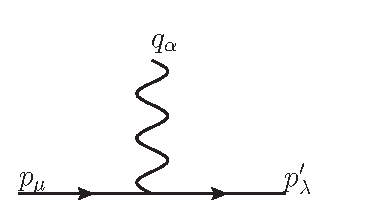
\includegraphics[scale=0.7]{eps/one-photon-fundamental} 
\end{minipage}
$ =  -ie[ g^{\mu\lambda}(p + p')^\alpha - g^{\lambda \alpha} (p' + [g-1]q)^\mu - g^{\alpha \mu} (p - [g-1]q)^\lambda ] $
}

\vspace{2em}


The part of the Lagrangian containing only the two photon terms:
\[
 \mathcal{L}_{A^2 } = \frac{e^2}{2} (A^\mu W^\nu - A^\nu W^\mu)^\dagger  (A_\mu W_\nu - A_\nu W_\mu) 
\]
\[
	= \frac{e^2}{2} \{ 2(W^\dagger \cdot W) (A^\dagger \cdot A)  - 2(W^\dagger \cdot A )(A^\dagger \cdot W) \}
\]

For the two-photon vertex, the term in the Lagrangian can be contracted two ways with the external photon field, so the corresponding diagram is:

\mbox{
\begin{minipage}{1.6in}
   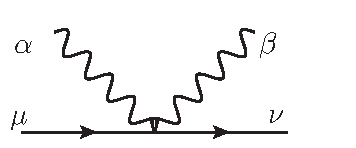
\includegraphics[scale=0.8]{eps/two-photon-fundamental} 
\end{minipage}
$	=	 -i e^2 ( 2 g^{\mu\nu} g^{\alpha \beta} - g^{\mu \beta} g^{\nu \alpha} - g^{\nu\beta}g^{\mu\alpha}) $
}

%TODO look up terminology here, make consistent with peskin
In addition to the vertices, there are rules for external legs.  External charged particle legs are replaced with the charged particle polarisation $\W_\mu$, while photon legs are replaced by $\epsilon_\mu$.  The polarisations $\W$ have three degrees of freedom, and obey the equation
\beq \label{eq:S1:pW}
	p \cdot \W(p) = 0
\eeq

\section{Relation between $\gv{\W}$ and $\phis$}
The amplitudes calculated in QED will involve the polarisations $\omega$, while those of NRQED will involve $\phis$.  Both represent the three degrees of freedom of a charged spin one particle, so a connection can be established between the two.

To determine how to write $\omega$ in terms of $\phis$, the current density of the two theories can be compared.  The current density \eqref{eq:S1:j0} for the relativistic theory was calculated in the previous chapter, while that of the nonrelativistic theory is just $\phis^\dagger \phis$.  

Now consider the current density in the case of $q=0$.  The identity $\hat{\partial}^\dagger = - \hat{\partial}$ is used.


%TODO clarify difference between derivative and derivative *operator* (add hats?)
\beqa
j_0
	&=& i\left\{	(\partial_0 W_\nu - \partial_\nu W_0)^\dagger W^{\nu} -  (\partial_0 W_\nu - \partial_\nu W_0) {W^{\dagger}}^\nu \right \}	\\
	&=& i\left\{	(\partial_0 W_i - \partial_i W_0)^\dagger W^{i} -  (\partial_0 W_i - \partial_i W_0) {W^{\dagger}}^i \right \}	\\
	&=& i\left \{  W^\dagger_i \partial_0^\dagger W^i - W^\dagger_0 \partial_i^\dagger W^{i} - {W^{\dagger}}^i \partial_0 W_i +{ W^{\dagger}}^i \partial_i W_0 \right \}	\\
	&=& i\left \{ -  W^\dagger_i \partial_0 W^i + W^\dagger_0 \partial_i W^{i}- {W^{\dagger}}^i \partial_0 W_i +{ W^{\dagger}}^i \partial_i W_0 \right \}	\\
	&=& i\left \{ - 2 W^\dagger_i \partial_0 W^i + W^\dagger_0 \partial_i  W^{i}+{ W^{\dagger}}^i \partial_i W_0 \right \}	\\
\eeqa

%FIXME really need to figure out terminology here
To express in terms of charged particle polarisations $\W$ and momentum $p$:
\[
\langle j_0(p) \rangle = 	- 2 \W^\dagger_i p_0 \W^i + \W^\dagger_0 p_i \W^{i} +{ \W^{\dagger}}^i p_i \W_0
\]
\[
	=	+ 2 p_0 \gv{\W}^\dagger \cdot \gv{\W} - \W^\dagger_0 \v{p} \cdot \gv{\W} - \gv{\W}^\dagger \cdot \v{p} \W_0
\]

$\W$ has four components but only three degrees of freedom.  The most sensible approach is to eliminate $\W_0$ by using \eqref{eq:S1:pW}.  Then $\W_0 = \frac{\gv{\W} \cdot \v{p}}{p_0}$, and the current density is
\[
	\langle j_0 \rangle = 2 p_0 \gv{\W}^\dagger \cdot \gv{\W} - 2 \frac{ ( \gv{\W}^\dagger \cdot \v{p})( \v{p} \cdot \gv{\W} )}{p_0} 
\]

Here the various components of $\W$ are mixed up.  As in the previous chapter, they can be disentangled by introducing spin matrices $\v{S}$.  Using the same identities as before, 
\[
	j_0 = 2p_0 \W^\dagger_i \left\{ \delta_{ij} - \frac{ \v{p}^2 \delta_{ij} - (\v{S} \cdot \v{p})^2_{ij} }{p_0^2} \right \} \W_j
\]
Then by demanding $j_0 = \phi^\dagger \phi$, a relation between $\phi$ and $\gv{\W}$ is found.
\[
 2p_0 \W^\dagger_i \left\{ \delta_{ij} - \frac{ \v{p}^2 \delta_{ij} - (\v{S} \cdot \v{p})^2_{ij} }{p_0^2} \right \} \W_j = \phi^\dagger \phi
\]
\[
	\gv{\W}  = \left\{ 2p_0 \left (1 - \frac{ \v{p}^2 - (\v{S} \cdot \v{p})^2 }{p_0^2}   \right ) \right \}^{-\frac{1}{2}} \phi
\]
To the order needed, this is
\beq \begin{split}
	\gv{\W} &= \frac{1}{\sqrt{2p_0}} \left (1 + \frac{ \v{p}^2 - (\v{S} \cdot \v{p})^2 }{2m^2} \right ) \phi	\\
	&=	 \frac{1}{\sqrt{2m}} \left (1 + \frac{ \v{p}^2}{4m^2} - \frac{(\v{S} \cdot \v{p})^2 }{2m^2} \right ) \phi
\end{split} \eeq


\section{Scattering off an external field in the relativistic theory}


The first step will be to do the calculations necessary to fix the one-photon terms in the NRQED Lagrangian.  This is done by considering the process of a single charged particle scattering off an external field, and calculating the amplitude in the relativistic theory.  

The one photon diagram, for incoming momentum $p$, outgoing $p'$ and photon momentum $q = p' - p$ is  
\beq	
	ie\left[ g^{\mu\nu} (p + p')^\lambda - g^{\nu\lambda}([g-1] q+p')^\mu + g^{\lambda\mu}([g-1] q-p)^\nu \right] 
\eeq

Contracted with external polarizations $\omin{\mu}$, $\omout{\nu}$ and external field $A_\lambda(q)$, this becomes
\beq
	ie\ \omin{\mu} \omout{\nu} \left[ g^{\mu\nu} (p + p')\cdot A - A^\nu ( [g-1] q+p')^\mu + A^\mu ( [g-1] q-p)^\nu \right]
\eeq

The W polarizations are subject to the condition that $ k \cdot \W(k) = 0 $.  This can be used to simplify the above expression, since then $p'^\mu \omin{\mu} = q^\mu \omin{\mu}$ and $p^\nu \omout{\nu} = -q^\nu \omout{\nu}$.  With this,  the vertex becomes

\beq
	ie\ \omin{\mu} \omout{\nu} \left[ g^{\mu\nu} (p + p')\cdot A  +g ( q^\nu A^\mu - q^\mu A^\nu ) \right] 	
\eeq

There are two terms here, one proportional to $g$ and one that has no $g$ dependence.  Call the first term, which doesn't depend on $g$
\beq
	\Mq = ie\ \omin{\mu} \omout{\nu} g^{\mu\nu} (p + p')\cdot A 
\eeq
and call the second 
\beq
	\Mg = ie g  \ \omin{\mu} \omout{\nu}  ( q^\nu A^\mu - q^\mu A^\nu ) 	
\eeq


%%% G independant one-photon terms
\subsection{Nonrelativistic expression for $M_q$}

Having written the amplitude as the sum of two terms, they must be cast in a form that can readily be compared with the NRQED result.  So, in terms of operators acting between $\phis^\dagger$ and $\phis$, and involving Galilean vectors and scalars.  The general strategy for each will be the same: first write in terms of $\W_i$ and then in terms of $\phis$.  Because the different components of $\W_i$ will be mixed up, as before it will be necessary to introduce spin matrices to express them as operators sandwiched between $\W^\dagger$ and $\W$.  Finally, derivatives of $A_\mu$ should be written in terms of $\v{E}$ and $\v{B}$ where possible.



The first term is 
\beqa
 \Mq 
 	&=& ie \omin{\mu} \omout{\nu}  g^{\mu\nu} (p + p')\cdot A			\\
	&=& ie (p + p')\cdot A ( \omin{0} \omout{0} - \omin{i} \omin{i})	\\
	&=&	ie [(p + p')\cdot A] \omout{j} \left( \frac{p'_j p_i}{p_0^2} - \delta_{ij} \right) \omin{i}	\\
	&=&	ie [(p + p')\cdot A] \gv{\W}^\dagger (p')  \left(  
			\frac{ \v{p} \cdot \v{p}' - (\v{S} \cdot \v{p})( \v{S} \cdot \v{p}') }{p_0^2}  -1 \right) \gv{\W}(p)
\eeqa
Since it is assumed that $q_0=0$, it follows that $p'_0 = p_0$.  In terms of the wave functions $\phis$ the above becomes
\beq
\Mq \approx 	-ie \frac{(p + p')\cdot A}{2p_0} \phis^\dagger
		\left( 1 + \frac{\v{p'}^2 - (\v{S}\cdot \v{p'})^2 }{2m^2} \right) 
		\left(1 - \frac{ \v{p} \cdot \v{p}' - (\v{S} \cdot \v{p})( \v{S} \cdot \v{p}')}{m^2} \right)
		\left( 1 + \frac{\v{p}^2 - (\v{S}\cdot \v{p})^2 }{2m^2} \right)
	\phis
\eeq
Simplifying this to the order needed
\beqa
\Mq &\approx&	-ie \frac{(p + p')\cdot A}{2p_0} \phi^\dagger
		\left( 1  + \frac{1}{2m^2} \left \{ \v{q} \cdot \v{p}' - (\v{S} \cdot \v{q})( \v{S} \cdot \v{p'})
			- \v{p} \cdot \v{q} + (\v{S} \cdot \v{p})( \v{S} \cdot \v{q}) \right \} \right )	
	\phi	\\
	&=& -ie \frac{(p + p')\cdot A}{2p_0} \phi^\dagger
		\left( 1  + \frac{1}{2m^2} \left \{ \v{q}^2 + [\v{S} \cdot \v{p}, \v{S} \cdot \v{q}] - (\v{S} \cdot \v{q})^2 \right \}
	 \right )\phi	\\
	&=& -ie \frac{(p + p')\cdot A}{2p_0} \phi^\dagger
		\left( 1  + \frac{1}{2m^2} \left \{ \v{q}^2 + i \v{S} \cdot \v{p} \times \v{q} - (\v{S} \cdot \v{q})^2 \right \}
	 \right )\phi
\eeqa

The outside factor involves a Lorentz dot product, and should be expressed in terms of Galilean quantities.  Again using that $p_0 = p'_0$:
\beq
	\frac{(p + p')\cdot A}{2p_0} = \frac{2p_0}{2p_0} A_0 - \frac{(\v{p} + \v{p'})\cdot \v{A} }{2p_0}
		= A_0 -  \frac{(\v{p} + \v{p'})\cdot \v{A} }{2p_0}
\eeq


Applying this to $M_q$, the result is:
\beq
\Mq = 	-ie  \phi^\dagger(p') \left( A_0  + \frac{A_0}{2m^2}( \v{q}^2 + i \v{S} \cdot \v{p} \times \v{q} - (\v{S} \cdot \v{q})^2 )
	- \frac{(\v{p} + \v{p'})\cdot \v{A} }{2p_0}
	- \frac{(\v{p} + \v{p'})\cdot \v{A} }{2m} \frac{i \v{S} \cdot \v{p} \times \v{q}}{2m^2} \right ) \phi(p)
\eeq

The NRQED result for the amplitude was written in position terms of $E$ and $B$, so it is necessary to express this result in the same sense.  A Fourier transform dictates that the transferred momentum $\v{q}$ becomes a derivative on the external field.  The prescription is $\v{q} \to -i \grad$.  The gauge has been chosen such that $E$ depends on $A_0$ terms only, and $B$ only upon $A_i$.  So it makes sense to consider such terms separately. 

%%% A_0 terms
\subsubsection{Transformation of $A_0$ terms in $\Mq$}
The second order term involving $A_0$ has both first and second derivatives of the potential.  The electric field is $E_i = -\partial_i A_0$ and so $q_i A_0 \to i E_i$.  Then $q_i q_j A_0 = \partial_j E_i = \partial_i E_j$.  Applying this to the higher order terms coupled to $A_0$:
\beq \label{eq:S1:A0Transforms}
A_0( \v{q}^2 + i \v{S} \cdot \v{p} \times \v{q} - (\v{S} \cdot \v{q})^2 )
	\to \grad \cdot \v{E} -  \v{S} \cdot \v{p} \times \v{E} - S_i S_j \grad_i E_j 
\eeq

%%% A_i terms
\subsubsection{Transformation of $\v{A}$ terms in $\Mq$}
The only term with derivatives of $\v{A}$ has the form $(\v{p} + \v{p'})\cdot \v{A}  (\v{S} \cdot \v{p} \times i\v{q})$.  This was worked out in \eqref{eq:Sh:A-p-id}, with the result (replacing $\sigma$ with $S$)
\beq  
(\v{p} + \v{p'}) \cdot \v{A}  (\v{S} \cdot \v{p} \times i\v{q} )
	= 2 \{  (\v{S} \cdot  \v{p})( \v{B} \cdot \v{p}) - \v{p}^2 \v{S} \cdot \v{B} \}
\eeq


%%% Total one-photon g-independant terms
\subsubsection{Total contribution of from $\Mq$ } 

So the first term in the vertex produces the following contribution to the scattering amplitude.
\beq  \begin{split}
	\Mq = ie \omin{\mu} \omout{\nu}  g^{\mu\nu} (p + p')\cdot A \to &
	 -ie \phi^\dagger(p') \Big ( A_0  + \frac{1}{2m^2}\{ \grad \cdot \v{E} -  \v{S} \cdot \v{p} \times \v{E} - S_i S_j \grad_i E_j \}
	\\& - \frac{\v{p}\cdot \v{A} }{p_0}
	+ \frac{1}{2m^3}\{ \v{p}^2 \v{S} \cdot \v{B} -  (\v{S} \cdot  \v{p})( \v{B} \cdot \v{p}) \} \Big )\phi(p)
\end{split}
\eeq


\subsection{Nonrelativistic expression for $\Mg$}
The second term looks like the external polarisations contracted with something like $F_{\mu\nu}$:
\beq
	\Mg = ie\ \omin{\mu} \omout{\nu} [g] ( q^\nu A^\mu - q^\mu A^\nu ) 	
\eeq
\subsubsection{General tensor type term}
Before calculating the specific term in question, consider the general type of term $\omout{\nu} \omin{\mu} u^\nu v^\mu$.  This should be expressed as a matrix element between the vector part of the polarization $\W$. 
\beqa
\omout{\nu} \omin{\mu} u^\nu v^\mu
	&=&	\W_0'  u_0 v_0 \W_0
		- (\v{\W}' \cdot \v{u}) v_0 \W_0
		- \W_0' u_0 (\v{v} \cdot \gv{\W}) 
		+ (\gv{\W'} \cdot \v{u})( \v{v} \cdot \gv{\W})	\\
	&=&	\frac{ \gv{\W'} \cdot \v{p'} u_0}{p'_0} \frac{ \gv{\W} \cdot \v{p} v_0}{p_0}
		- (\v{\W}' \cdot \v{u}) \frac{ \gv{\W} \cdot \v{p} v_0}{p_0}
		- \frac{ \gv{\W'} \cdot \v{p'} u_0}{p'_0}  (\v{v} \cdot \gv{\W}) 
		+ (\gv{\W'} \cdot \v{u})( \v{v} \cdot \gv{\W})	\\
	&=&	\gv{\W}'_j \left (
			\frac{ u_0 v_0}{p_0 p'_0} p'_j p_i
			- \frac{v_0}{p_0} u_j p_i
			- \frac{u_0}{p'_0} p'_j v_i
			+ u_j v_i
		\right ) \W_i	\\
	&=&	\gv{\W'}^\dagger \left (
			\frac{ u_0 v_0}{p_0 p'_0} [ \v{p} \cdot \v{p'} - (\v{p} \cdot \v{S}) (\v{p'} \cdot \v{S}) ]
			- \frac{v_0}{p_0} [ \v{p} \cdot \v{u} - (\v{p} \cdot \v{S}) (\v{u} \cdot \v{S}) ] \right.
	\\&&		\left. - \frac{u_0}{p'_0} [ \v{v} \cdot \v{p'} - (\v{v} \cdot \v{S}) (\v{p'} \cdot \v{S}) ]
			+ [ \v{v} \cdot \v{u} - (\v{v} \cdot \v{S}) (\v{u} \cdot \v{S}) ]
		\right ) \gv{\W}	\\
\eeqa

\subsubsection{$\Mg$ term}

Now that identity can be used to calculate $\Mg$ with $q_0=0$ (and thus $p'_0 = p_0)$.

\beqa
\Mg
	&=&	+ie g\gv{\W'}^\dagger \Bigg(
			-\frac{A_0}{p_0} \left\{ \v{p} \cdot \v{q} - (\v{p} \cdot \v{S}) (\v{q} \cdot \v{S}) \right\}
			+ \frac{A_0}{p_0} \left\{ \v{q} \cdot \v{p'} - (\v{q} \cdot \v{S}) (\v{p'} \cdot \v{S}) \right\}
	\\&&		+\left\{ \v{q} \cdot \v{A} - (\v{A} \cdot \v{S}) (\v{q} \cdot \v{S}) \right\}
			-\left\{ \v{A} \cdot \v{q} - (\v{q} \cdot \v{S}) (\v{A} \cdot \v{S}) \right\}
		\Bigg) \gv{\W}	\\
	&=&	+ie g\gv{\W'}^\dagger \left\{
			\frac{A_0}{p_0} \Big( \v{q}^2 - (\v{q} \cdot \v{S} )^2 + [\v{p} \cdot \v{S}, \v{q} \cdot \v{S}] \Big)
			- [\v{A} \cdot \v{S}, \v{q} \cdot \v{S}]
		\right\} \gv{\W}
\eeqa

Next replace $\W$ with $\phis$ and rewrite in terms of $E$ and $B$.  Again, it makes sense to treat terms with $A_0$ and $A_i$ separately. 
%%% A_0 terms
\subsubsection{Transformation of $A_0$ terms in $\Mg$}
The first term coupled to $A_0$ is already second order, so only the first order approximation for $\W$ is needed: $\v{\W} \approx \frac{1}{\sqrt{2m}}\phi$
\beq
	\Mg^E = ie g\phi^\dagger(\v{p'})   \frac{A_0}{2m^2} \left( \v{q}^2 - (\v{q} \cdot \v{S} )^2 + i\v{S} \cdot \v{p} \times \v{q} \right) \phi (\v{p})
\eeq
This is exactly the same structure that arose in working with $\Mq$.  From \eqref{eq:S1:A0Transforms} it is:
\beq
\Mg^E = 
 ie g \frac{1}{2m^2}\phi^\dagger(\v{p'})  ( \grad \cdot \v{E} -  \v{S} \cdot \v{p} \times \v{E} - S_i S_j \grad_i E_j ) \phi (\v{p})
\eeq

%%% A_i terms
\subsubsection{Transformation of $\v{A}$ terms in $\Mg$}
The second term  is  $\Mg^B = -ie g\gv{\W^\dagger} [\v{A} \cdot \v{S}, \v{q} \cdot \v{S}] \gv{\W}$.  The commutator is:
\beq
[\v{A} \cdot \v{S}, \v{q} \cdot \v{S}]
	=	A_i q_j [S_i, S_j]	
	=	A_i q_j (i\epsilon_{ijk} S_k)	
	=	- \v{S} \cdot i\v{q} \times \v{A}	
\eeq
In terms of $B$ this yields
\beqa
- \v{S} \cdot i\v{q} \times \v{A}
	&\to&	- \v{S} \cdot \grad \times \v{A} 	\\
	&=&	-\v{S} \cdot \v{B}	
\eeqa
So the whole thing is $ieg \gv{\W^\dagger} (\v{S} \cdot \v{B}) \gv{\W}$.  This is first order so corrections to this term, coming from the expression for $\W$ in terms of $\phi$, are needed.

\beq
 \Mg^B = ieg\gv{\W^\dagger} (\v{S} \cdot \v{B}) \gv{\W} \to
	ieg \frac{1}{2p_0} \phi^\dagger
		\left( 1 + \frac{\v{p'}^2 - [\v{S}\cdot \v{p'}]^2 }{2m^2} \right) 
		\v{S} \cdot \v{B}
		\left( 1 + \frac{\v{p}^2 - [\v{S}\cdot \v{p}]^2 }{2m^2} \right)
	\phi
\eeq


Since the $B$ field is constant, all terms with $q$ vanish, so the above reduces to
\beq
\Mg^B	=  ieg \frac{1}{2p_0} \phi^\dagger	\left(  
		\v{S} \cdot \v{B} +  \v{S} \cdot \v{B} \frac{p^2}{2m^2} + \frac{1}{2m^2}\left\{ \v{S} \cdot \v{B}, \frac{\v{p}^2}{2} - [\v{S}\cdot \v{p}]^2 \right\}_+	\right ) \phi
\eeq
Expanding $\frac{1}{2p_0} = \frac{1}{2m}(1 - \frac{\v{p}^2}{2m^2} )$ eliminates the second term:
\beq
	\Mg^B =  ieg \frac{1}{2m} \phi^\dagger	\left(  
		\v{S} \cdot \v{B}  + \frac{1}{2m^2}\left\{ \v{S} \cdot \v{B}, \frac{\v{p}^2}{2} - [\v{S}\cdot \v{p}]^2 \right\}_+	\right ) \phi
\eeq



This anticommutator actually occurred as part of the previous calculation of the spin-one Hamiltonian.  From \eqref{eq:A:SBanticom}:

\beq
\frac{1}{2m^2}\left \{ \frac{\v{p}^2}{2} - (\v{S} \cdot \v{p})^2, \v{S} \cdot \v{B} \right \} = -\frac{(\v{S} \cdot \v{p})( \v{B} \cdot \v{p})}{2m^2}
\eeq
Using that, the part of $\Mg$ which contains $\v{A}$ reduces to 
\beq
\Mg^B = 	ieg \frac{1}{2m}\phi^\dagger \left( \v{S} \cdot \v{B} - \frac{(\v{S} \cdot \v{p})( \v{B} \cdot \v{p})}{2m^2}  \right) \phi
\eeq

\subsubsection{Total contribution of $\Mg$}
Now the total contribution of the second $g$-dependent term to the scattering amplitude is:
\beq
\begin{split}
\Mg	=	ieg \frac{1}{2m}\phi^\dagger \Big ( \v{S} \cdot \v{B} - \frac{(\v{S} \cdot \v{p})( \v{B} \cdot \v{p})}{2m^2}  
		+ \frac{1}{m} \left\{ \grad \cdot \v{E} -  \v{S} \cdot \v{p} \times \v{E} - S_i S_j \grad_i E_j \right \} \Big ) \phi
\end{split}
\eeq



%%%%%%%%% ALL TERMS TOGETHER  %%%%%%%%%%%%%
\subsection{All terms together}
Having expressed each of the terms, the total scattering amplitude, as calculated in the relativistic theory, is found simply by adding them together.  (Elastic scattering off an external field, with constant $\v{B}$.)

First consider the terms related to the electric field/potential:
\beq
M^E =  	-ie\phi^\dagger \left( A_0  - (g-1)  \frac{1}{2m^2} \{ \grad \cdot \v{E} -  \v{S} \cdot \v{p} \times \v{E} - S_i S_j \grad_i E_j \} \right) \phi
\eeq
The terms with bare $\v{A}$:
\beq
M^A = ie\phi^\dagger \left( \frac{\v{p}\cdot \v{A} }{p_0}\right ) \phi 
	\approx
ie\phi^\dagger \left( \frac{\v{p}\cdot \v{A} }{m} - \frac{\v{p}\cdot \v{A} \v{p}^2}{2m^3}\right ) \phi 
\eeq

Then the terms with $B$ in them:
\beq
M^B = 	i\frac{e}{2m}\phi^\dagger \left(  
		g \v{S} \cdot \v{B} -  \v{S} \cdot \v{B} \frac{\v{p}^2}{m^2}
		-\frac{g-2}{4m^2}(\v{S} \cdot \v{p} )( \v{B} \cdot \v{p})
	\right ) \phi
\eeq
So to the desired order, the amplitude for scattering off an external field, as calculated from relativistic theory, is
\beq \label{eq:S1:MRel}
\begin{split}
iM_{REL} =& -ie \phi^\dagger \Big (
		 A_0  - \frac{\v{p}\cdot \v{A} }{m} + \frac{\v{p}\cdot \v{A} \v{p}^2}{2m^3}
		- \frac{g-1}{2m^3}\{ \grad \cdot \v{E} -  \v{S} \cdot \v{p} \times \v{E} - S_i S_j \grad_i E_j \}
		\\& - g\frac{1}{2m} \v{S} \cdot \v{B}
		+ \v{S} \cdot \v{B} \frac{\v{p}^2}{2m^3}
		+ \frac{g-2}{4m^3}(\v{S} \cdot \v{p} )( \v{B} \cdot \v{p})
	\Big ) \phi
\end{split}
\eeq



\section{Compton scattering in the relativistic theory}


The previous calculation is enough to fix all the coefficients of the NRQED lagrangian.  Just like for spin one-half, however, calculating the the coefficients of some two-photon terms will help check the consistency of the approach.  And as before, the two photon coefficients may be fixed by calculating the amplitude for Compton scattering in the relativistic theory.  

In the spin one-half case, there was only one type of electromagnetic vertex, representing the interaction of a single photon with an electron line.  So the process of Compton scattering (at the leading orders) was determined entirely by diagrams composed of this vertex.  In the spin one Lagrangian, however, there are also four particle vertices involving two photons. 

So here there are two types of contributions, one from the fundamental two-photon vertex and the other from the combination of two one-photon vertices.  Two-photon contact terms in the Lagrangian will have an additional symmetry factor of 1/2 compared to the expression for the vertex. 

\begin{minipage}{1in}
   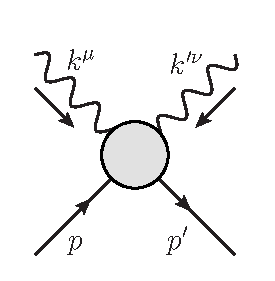
\includegraphics[scale=0.7]{eps/blob1} 
\end{minipage}
$=$
\begin{minipage}{1.6in}
   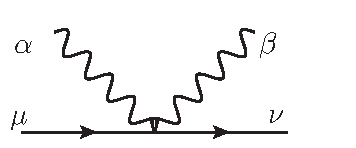
\includegraphics[scale=0.7]{eps/two-photon-fundamental} 
\end{minipage}
$+$
\begin{minipage}{1.6in}
   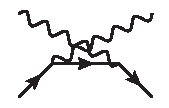
\includegraphics[scale=1]{eps/crossed-small} 
\end{minipage}
$+$
\begin{minipage}{1.6in}
   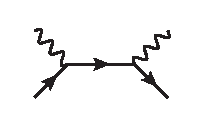
\includegraphics[scale=1]{eps/uncrossed-small} 
\end{minipage}


To define conventions for this calculation, say that the incoming charged particle has momentum $p$, and the outgoing, momentum $p'$.  Define both photon momenta $k$ and $k'$ going \emph{into} the vertex or vertices.  Charged particle polarisations are $\W$, while photon polarisations are $\A$.

Once scattering amplitude has been calculated in terms of relativistic quantities, it must be compared to the NRQED vertices.  The process is the same as for the calculation of the one-photon process.  First, write all terms "sandwiched" between $\W^\dagger$ and $\W$.  Some terms will already be proportional to $\gv{\W^\dagger} \cdot \gv{\W}$.  But there will be others of the form $[\gv{\W^\dagger} \cdot \v{u}] [\v{v} \cdot \gv{\W}]$.  To deal with these the spin matrices $\v{S}$ are introduced, with the identity:
\[
	(\gv{\W^\dagger} \cdot \v{u}) (\v{v} \cdot \gv{\W}) = \W^\dagger_a \left( \delta_{ab} \v{u} \cdot \v{v} - v_i u_j\{S_i S_j\}_{ab}  \right) \W_b
\]

%TODO is this too redundant?
The charged particle polarisations must be replaced by the Schrodinger-like wave functions $\phi$.  Consistent with the calculations for the one-photon terms, the prescription is:
\[
	\gv{\W}(p) \to \frac{1}{\sqrt{2m}}\left( 1 + \frac{\v{p}^2}{4m^2} - \frac{ [\v{S}\cdot \v{p}]^2 } {2m^2} \right)\phis(\v{p})
\]




\subsection{Two-photon vertex}

%TODO add diagram?
The relativistic two-photon vertex is

\VertexEq{two-photon-fundamental}{
 -i e^2 ( 2 g^{\mu\nu} g^{\alpha \beta} - g^{\mu \beta} g^{\nu \alpha} - g^{\mu \alpha} g^{\nu \beta} )
}

The contribution of this diagram to Compton scattering is, contracting with the photon and charged particle polarisations:
\beq
\Mcontact = 
	 -i e^2( 2[\W^\dagger \cdot \W][\Adag \cdot \A] - [\W^\dagger \cdot \A] [ \W \cdot \Adag]  -[\W^\dagger \cdot \Adag] [ \W \cdot \A] )
\eeq

%TODO fix middle terms
%Expanding this, using the identity $\W_0 = \frac{\gv{\W} \cdot \v{p}}{p_0}$, and keoming only the needed order:
%\[
%	2 i e^2 \gv{\W^\dagger} \cdot \gv{\W} (\A_0 \A_0' - \v{\A}' \cdot \v{\A} ) 
%	- 2 i e^2 \frac{\A_0'}{m} (\gv{\W^\dagger} \cdot \v{\A} ) ( \v{p} \cdot \gv{\W} )
%	- 2 i e^2 \frac{\A_0}{m} (\gv{\W^\dagger} \cdot \v{p'}) (\v{\Adag} \cdot \gv{\W} )
%	+ i e^2 (\gv{\W^\dagger} \cdot  \v{\A}) (\v{\Adag} \cdot \gv{\W})
%	+ i e^2 (\gv{\W^\dagger} \cdot  \v{\A}) (\v{\Adag} \cdot \gv{\W})		
%\]



In calculating a physical process, the result will not depend upon the gauge.  To simplify the calculation, choose a gauge where $\A_0 = 0$ and use the identity $\W_0 = \frac{\gv{\W} \cdot \v{p}}{p_0}$.  Then the above reduces to
\beq
\Mcontact =  -2 i e^2 (\gv{\W^\dagger} \cdot \gv{\W}) (\v{\A}' \cdot \v{\A}) 
	+  i e^2 (\gv{\W^\dagger} \cdot  \v{\A}) (\v{\Adag} \cdot \gv{\W})	
	+  i e^2 (\gv{\W^\dagger} \cdot  \v{\Adag}) (\v{\A} \cdot \gv{\W})	
\eeq



\subsection{Terms arising from two vertex diagrams}

The diagrams with two vertices contribute not just to the point-like interaction, but also the part of the scattering amplitude corresponding to two vertex diagrams in NRQED.  By decomposing the relativistic propagator, the local and nonlocal terms can be separated.  This is exactly analogous to what was done for the spin one-half case, but the structure of both  the propagator and the sums over intermediate states differ.  

%Main calculation
\subsubsection{Dealing with the relativistic propagator}

The relativistic propagator will be decomposed into the sum of two pole terms and a constant term.  The numerators of the two pole terms are usefully expressed as a sum over intermediate on-shell states i.e. a sum over polarisations. If $a$ indexes the three orthogonal polarisation states, and $\ell$ is some on-shell momentum, then this sum is
\beq
	\sum_a \W_a^\mu(\ell) \W_a^\nu(\ell) = \frac{\ell^\mu \ell^\nu}{m^2} - g^{\mu\nu} 
\eeq
It's convenient to define for some arbitrary (\emph{not} necessarily on mass shell) momentum $k$
\beq
  G^{\mu\nu}(k) = g^{\mu\nu} - \frac{k^\mu k^\nu}{m^2}
\eeq

The idea is that the two parts of the propagator with poles represent two types of processses, one involving intermediate particles, the other intermediate anti-particles.  These particles are to be considered on-shell, so it is useful to define Lorentz four vectors which represent the momentum of on-shell particles and anti-particles.  For the particles, let $\qp = (\sqrt{\v{q}^2+m^2}, \v{q})$.   And for the antiparticles, let $\qm = (-\sqrt{\v{q}^2+m^2}, \v{q})$.  Also define $E_q = \sqrt{\v{q}^2+m^2}$.

The relativistic propagator to be decomposed is
\beq
	i\frac{  \frac{q^\mu q^\nu}{m^2} - g^{\mu\nu} }{q^2 - m^2} = \frac{ - i G^{\mu\nu}(q) }{q^2 - m^2}
\eeq

Here $q$ is no on mass-shell.  This will be written as the sum of two pole terms, having as their numerator a sum over intermediate on mass-shell states.  In comparison to the spin one-half case, there will be an additional constant which for now can be called $x^{\mu\nu}$.
\[
	\frac{ -i G^{\mu\nu}(q) }{q^2 - m^2} = \frac{1}{2 \E{q}} \left(  \frac{ -i G^{\mu\nu}(\qp)  }{q_0 - \E{q} } - \frac{ -i G^{\mu\nu}(\qm)  }{q_0 + \E{q} } \right) + i x^{\mu\nu}
\]

Explicit calculation shows that $x^{\mu\nu}=1/m^2$ when $\mu=\nu=0$, but is zero otherwise.  So $x^{\mu\nu} = g^{\mu0} g^{\nu0} /m^2$, and the relativistic propagator can be written as
\[
	\frac{ -i G^{\mu\nu}(q) }{q^2 - m^2} = \frac{i}{2 \E{q}} \left(  \frac{ -G^{\mu\nu}(\qp)  }{q_0 - \E{q} } - \frac{ -G^{\mu\nu}(\qm)  }{q_0 + \E{q} } \right) + i\frac{g^{\mu0} g^{\nu0}}{m^2}
\]

%Relevancy
The reason for this decomposition is that only the part of the propagator which gives rise to the point-like interaction is needed.  Other contributions to the scattering amplitude in the nonrelativistic theory come from diagrams involving two one-photon vertices.  At the necessary order these are exactly the $1/(q_0 - \E{q})$ terms.  So the point-like interactions can be obtained by simply dropping these terms.  After this, rewriting the amplitude in terms of nonrelativistic quantities will still be necessary.


From the full propagator, define the needed part $P^{\mu\nu}$ as outlined above.

\beq
	P^{\mu\nu} =    \frac{i}{2 \E{q}} \frac{ G^{\mu\nu}(\qm)  }{q_0 + \E{q} } + i\frac{g^{\mu0} g^{\nu0}}{m^2}
\eeq
This is just the propagator without the nonlocal terms.
%Approximation

All that is needed for the final result are the leading order terms, and those with one additional power of momentum.  So $E_q  \approx m$.  $q_0$ is the off-mass shell energy of the propagator, but in this nonrelativistic scenario it will be close to $m$.  So write $q_0 + E_q \approx 2m + [q_0-m]$ and then use that $[q_0-m]$ is small.
\[
	P^{\mu\nu} \approx   \frac{1}{2m} \frac{i G^{\mu\nu}(\qm)  }{2m + [q_0-m]} + i\frac{g^{\mu0} g^{\nu0}}{m^2}
			\approx \left( 1 - \frac{[q_0-m]}{2m} \right )\frac{ i G^{\mu\nu}(\qm)  }{4m^2} + i \frac{g^{\mu0} g^{\nu0}}{m^2}
\]

Consider now $G^{\mu\nu}(\qm) = g^{\mu\nu} - \frac{\qm^\mu \qm^\nu}{m^2}$.  Using $\qm_0 \approx -m$ it follows that

\[
	G^{00} = (1 - \frac{\qm^0 \qm^0}{m^2} \approx  0
\]

\[
	G^{0i} = G^{i0} =  - \frac{\qm^0 \qm^i}{m^2} \approx  \frac{q^i}{m}
\]


\[
	G^{ij} = \delta^{ij} - \frac{\qm^i \qm^j}{m^2} \approx \delta^{ij}
\]

So the different components fo $P^{\mu\nu}$ are, to the order needed.

\beqa \label{eq:S1:Pvalues}
 P^{00} &=& \frac{i}{m^2} 	\\
 P^{0i} &=& P^{i0} = i\frac{  q^i  }{4m^3}		\\
 P^{ij} &=& - \left(1 - \frac{q_0 - m}{2m} \right )\frac{i \delta^{ij} }{4m^2} 	
\eeqa


\subsubsection{Vertex calculations}

There are two tree diagarms, crossed and uncrossed.  Each consists of a propagator and two vertices contracted with external fields.  In the previous section the propagator was considered; the result is that it may simply be replaced by the above quantities $P^{\mu\nu}$ to compare with the local vertices of NRQED.    Now the part of the calculation involving the vertices is considered.

Use $V$ and $\overline{V}$ to represent the vertices of the uncrossed diagram, and $U$, $\overline{U}$ for the crossed.  These can be defined in terms of vertex diagrams, the external lines contracted with polarisations.

%FIXME diagrams -- wrong polarisation states
$V_\lambda = $
\begin{minipage}{1in}
   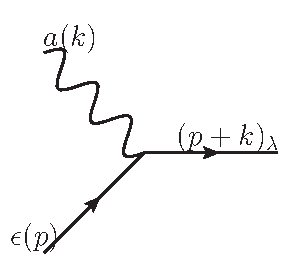
\includegraphics[scale=0.7]{eps/V-lambda} 
\end{minipage}
\hspace{8em}
$\overline{V}_\rho = $
\begin{minipage}{1in}
   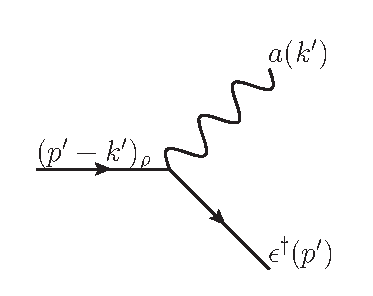
\includegraphics[scale=0.7]{eps/V-bar-rho} 
\end{minipage}



$U_\lambda = $
\begin{minipage}{1in}
   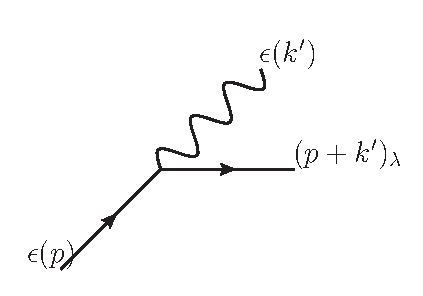
\includegraphics[scale=0.7]{eps/U-lambda} 
\end{minipage}
\hspace{8em}
$\overline{U}_\rho = $
\begin{minipage}{1in}
   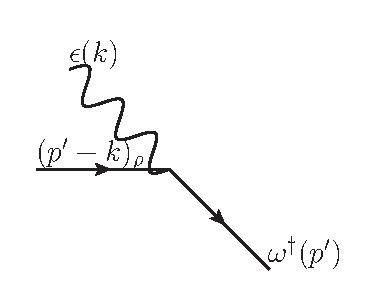
\includegraphics[scale=0.7]{eps/U-bar-rho} 
\end{minipage}

With the above definitions it is clear that the point-like interactions, taken from the two diagrams, will be

\begin{minipage}{1in}
   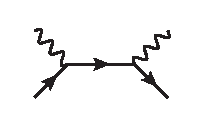
\includegraphics[scale=1]{eps/uncrossed-small} 
\end{minipage}
$ \to \overline{V}_\rho P^{\rho \lambda}(p+k) V_\lambda$
\hspace{5em}
\begin{minipage}{1in}
   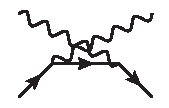
\includegraphics[scale=1]{eps/crossed-small} 
\end{minipage}
$ \to \overline{U}_\rho P^{\rho \lambda}(p+k') U_\lambda$



Only terms one past leading order are needed to fix the coefficient of the $\v{S} \cdot \v{E} \times \v{A}$ term in NRQED.  So tabulate the first two orders of each vertex for time and spatial components separately.  




The basic vertex inside $V_\lambda$ is, with incoming particle momentum $p^\mu$, incoming photon momentum $k^\alpha$ and outgoing $(p+k)^\lambda$:

\[
	ie[ g^{\mu\lambda}(2p + k)^\alpha - g^{\lambda \alpha} (p + [g]k)^\mu - g^{\alpha \mu} (p-[g-1]k)^\lambda ]
\]

Contracted with external charged particle and photon polarizations $\W_\mu$ and $\A_\alpha(k)$ gives:
\[
	V_\lambda = ie[\W^\lambda (2p + k) \cdot \A - \A^\lambda (p+[g]k) \cdot \W - \A \cdot \W (p-[g-1]k)^\lambda ]
\]
  
The other three vertices can be obtained simply by substituting the appropriate momenta and polarisations.  For instance, the similar vertex for outgoing momentum $(p+k)^\rho = (p' - k')^\rho$, photon $k'$, and final momentum $p'$ is

\[
	\overline{V}_\rho = ie[\W^{\dagger\rho} (2p' - k') \cdot \Adag - \A^\rho (p'-[g]k') \cdot \W^\dagger  - \Adag \cdot \W^\dagger  (p'+[g-1]k')^\rho ]
\]
So $\overline{V}_\rho$ can be obtained by just substituting $\W^\dagger$ for $\W$, $p'$ for $p$, and $-k'$ for $k$.  With this in mind, only the calculation for $V_\lambda$ need be explicitly performed, since all four have the same form.



%%%%%%%%%%%%%%%%%%%%%%%%%%%%%%%%%%%%%%
\subsubsection{Calculation of $V_\lambda$}
In calculating the two photon vertex, the gauge was chosen such that $\A_0=0$.  This will help simplify the calculation.  Also, only the first two orders are needed.

The leading order terms must have only the time-component of the charged particles momentum: the on mass-shell $p_0 = p'_0 \approx m$.  Corrections to $p_0$ do not enter at the necessary level of approximation for the two photon diagrams. 

The next to leading order terms have exactly one power of external momentum $\v{p}$ or photon momentum $\v{k}$, $\v{k'}$ or $k_0$, $k'_0$.  Any term containing $\W_0$ is of at least this order, since $\W^0(p) \approx \frac{\gv{\W} \cdot \v{p}}{m}$.

With these considerations, the vertex $V$ can now be explicitly calculated, treating $V_0$ and $V_i$ separately.

\paragraph{The $V_0$ term}
Consider first the time-component of $V$.  It has three parts --- label them $T_0^N$.
\beq 
	V_0 = ie[ \underbrace{\W^0 (2p + k) \cdot \A }_I 
			- \underbrace{\A^0 (p+[g]k) \cdot \W }_{II}
			- \underbrace{\A \cdot \W (p-[g-1]k)^0}_{III} ]
\eeq	

Up to some outer factor the first term is then $\W^0 (2p + k) \cdot \A$.  Since $\W^0 =\frac{\gv{\W} \cdot \v{p}}{m}$ this becomes
\beq
T_0^I = \W^0 (2p + k) \cdot \A = \frac{\gv{\W} \cdot \v{p}}{m} (2p + k) \cdot \A  = 2 \frac{\gv{\W} \cdot \v{p}}{m} p_0  \A_0 + \mathcal{O}(\frac{p^2}{m})
\eeq

The spatial component of $\A$ only appears with an additional power of momentum and so is too high order, and the $\A_0$ term vanishes in the chosen gauge.  So this term doesn't actually contribute at all to the result:
\beq
T^{I}_0 = \W^0 (2p + k) \cdot \A \sim \mathcal{O}(\frac{p^2}{m})
\eeq

%Term 2
The second term goes as $ -\A^0 (p+[g]k) \cdot \W$.   Obviously with the choice of gauge this doesn't contribute either.
\beq
	T^{II}_0 = 0
\eeq	
% (Unneeded calculation in this gauge) Expanding the dot product we can use that $p \cdot \W = 0$ leaving only $k \cdot \W = -\v{k} \cdot \gv{\W}$.
%\[	-\A_0 (2k) \cdot \W = 2 \A_0 \v{k} \cdot \gv{\W} \]

%Term 3
The final term here is $- \A \cdot \W (p-[g-1]k)^0 $  Expanding the dot product and again using the choice of gauge
\beq
	T^{III}_0 = - \A \cdot \W (p-[g-1]k)^0   \approx - (\A_0 \W_0  - \v{\A} \cdot \gv{\W} ) (m - [g-1]k_0) = (m-[g-1]k_0)\v{\A} \cdot \gv{\W}
\eeq

%Sum
That is the only contribution to the $\lambda=0$ vertex, so the total is just 
\beq \label{eq:S1:V0vertex}
	V_0 = ie(m-[g-1]k_0)\v{\A} \cdot \gv{\W}
\eeq

\paragraph{The $V_i$ term}
Now look at the spatial component, which again has three parts which can be labelled $T^N_i$.
\beq
 V_i = ie[ \underbrace{\W^i (2p + k) \cdot \A}_I
 	 - \underbrace{\A^i (p+[g]k) \cdot \W}_{II}
 	  - \underbrace{\A \cdot \W (p-[g-1]k)^i}_{III} ]
\eeq

% Term 1
The first term is simply
\beq
	T_i^I = \W^i (2p + k) \cdot \A = \W^i ([2m + k_0]\A_0 - [2\v{p} + \v{k}] \cdot \v{\A} ]) 
\eeq

Which after applying the gauge conditions becomes
\beq
	T_i^I =  \W^i (2p + k) \cdot \A =  - 2 (\v{p} \cdot \v{\A} ) \W^i 
\eeq

%Term 2 \v{A} \cdot \gv{\W}	
For the second term $- \A^i (p+2k) \cdot \W$, again use that $p \cdot \W=0$ so 
\beq
	T_i^{II} = - \A^i (p+[g]k) \cdot \W \approx g \A^i \v{k} \cdot \gv{\W} 
\eeq
%Term 3
And in the third term $ - \A \cdot \W (p-[g-1]k)^i$, the $\A_0$ term is of too high order (irregardless of the gauge), leaving
\beq
	T_i^{III} = - \A \cdot \W (p-[g-1]k)^i \approx \v{\A} \cdot \gv{\W} (p-[g-1]k)^i
\eeq
All three terms together give
\beq \label{eq:S1:Vivertex}
V_i = ie\left( [g]\v{k} \cdot \gv{\W} \A^i - 2\v{p} \cdot \v{\A} \W^i + \v{\A} \cdot \gv{\W} [p - [g-1]k]^i \right )
\eeq

\paragraph{Tabulation of results}

So of course parallel calculations for the other vertices could be done, as previously mentioned it is easier to note that they have the same general for.  To obtain $\overline{V}$ the recipe is that $p \to p'$, $k \to -k'$, $\W \to \W^\dagger$.  Similar considerations work for $U$, where the only difference is that because of the crossed lines, $k$ and $k'$ are swapped.

If $V$ is considered as a function of $p$, $k$ and $\W$: $V_\mu(p, k, \W)$,  then 
\beqa
	\overline{V}_\mu &=& V_\mu(p', -k',  \W^\dagger)	\\
	U_\mu &=& V_\mu(p, k',  \W)			\\
	\overline{U}_\mu &=& V_\mu(p', -k, \W^\dagger)	\\
\eeqa





Only the first two orders are needed, so for each type of vertex write $X^{(1)}$ to indicate a leading order terms, and $X^{(2)}$ to indicate next to leading order terms.

The vertex $V$ was explicitly calculated, the results are
\beqa
	V_0^{(1)} &=&	i e m \v{\A} \cdot \gv{\W}			\\
	V_0^{(2)} &=&	-i e [g-1] k_0  \v{\A} \cdot \gv{\W} 	\\
	V_i^{(1)} &=&	0				\\
	V_i^{(2)} &=&	 ie\left( [g]\v{k} \cdot \gv{\W} A^i - 2\v{p} \cdot \v{\A} \W^i + \v{\A} \cdot \gv{\W} [p - [g-1]k]^i \right )	\\
\eeqa

$\overline{V}$ is obtained from $V$ as explained above:
\beqa
	\overline{V}_0^{(1)} &=&	i e m \v{\Adag} \cdot \gv{\W^\dagger}			\\
	\overline{V}_0^{(2)} &=&	i e [g-1] k'_0 \v{\Adag} \cdot \gv{\W^\dagger}			\\
	\overline{V}_i^{(1)} &=&	0								\\
	\overline{V}_i^{(2)} &=&	i e ( -[g]\v{k'} \cdot \gv{\W^\dagger} {\Adag}^i - 2\v{p'} \cdot \v{\Adag} \W^{\dagger^i}
				+ \v{\Adag} \cdot \gv{\W^\dagger} [p' + [g-1]k']^i )	\\
\eeqa

Using $U$ to denote the vertices of the crossed diagram, the first is:
\beqa
	U_0^{(1)} &=&	i e m \v{\Adag} \cdot \gv{\W}			\\
	U_0^{(2)} &=&	-i e [g-1] k'_0  \v{\Adag} \cdot \gv{\W} 	\\
	U_i^{(1)} &=&	0				\\
	U_i^{(2)} &=&	 i e \left( [g]\v{k'} \cdot \gv{\W} \Adag^i - 2\v{p} \cdot \v{\Adag} \W^i + \v{\Adag} \cdot \gv{\W} [p - [g-1]k']^i \right )	\\
\eeqa

And for the second:
\beqa
	\overline{U}_{0}^{(1)} &=&	i e m \v{\A} \cdot \gv{\W^\dagger}			\\
	\overline{U}_{0}^{(2)} &=&	i e [g-1] k_0 \v{\A} \cdot \gv{\W^\dagger}			\\
	\overline{U}_{i}^{(1)} &=&	0								\\
	\overline{U}_{i}^{(2)} &=&	i e ( -[g]\v{k} \cdot \gv{\W^\dagger} {\A}^i - 2\v{p'} \cdot \v{\A} \W^{\dagger^i}
				+ \v{\A} \cdot \gv{\W^\dagger} [p' + [g-1]k]^i )	\\
\eeqa
In addition to the vertices, the final result will involve the propagator terms which were, as previously derived:
\beqa
 P^{00} &=& \frac{i}{m^2} 	\\
 P^{0i} &=& P^{i0} = i\frac{  q^i  }{4m^3}		\\
 P^{ij} &=& - \left(1 - \frac{q_0 - m}{2m} \right )\frac{i \delta^{ij} }{4m^2} 	
\eeqa
Above, $q = p+k$ for the uncrossed diagrams, and $q = p+k'$ for crossed.  It turns out that for this particular calculation, only $P_{00}$ will contribute.  And since at the needed order only the pure contact term contributes, the momentum dependence of the propagator doesn't show up in the final result.

 
From the above pieces can be calculated the point-like terms which arise from the two-vertex diagram.  Including both crossed and uncrossed diagrams, the contact part that arises is:

\begin{minipage}{1in}
   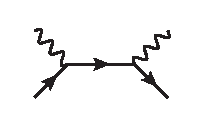
\includegraphics[scale=1]{eps/uncrossed-small} 
\end{minipage}
\hspace{1em}$+$
\begin{minipage}{1in}
   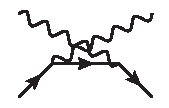
\includegraphics[scale=1]{eps/crossed-small} 
\end{minipage}
$
	\to \overline{V}_\rho P^{ \rho \lambda}(p+k) V_\lambda +   \overline{U}_\rho P^{ \rho \lambda}(p+k') U_\lambda
$

\subsection{Two vertex contribution}

Each piece has been calculated, it is now just a matter of putting it all together.
\subsubsection{Leading order}
The leading order term from uncrossed diagrams will be $V_\lambda^{(1)} P^{\lambda \rho} \overline{V}_\rho^{(1)}$, or
\beqa
V_{\lambda=0}^{(1)} P^{00} \overline{V}_{0}^{(1)} + V_{i}^{(1)} P^{ij} \overline{V}_{j}^{(1)}	
	&=&	-e^2 m^2 \gv{\W^\dagger} \cdot \v{\Adag} \frac{i}{m^2}\v{\A} \cdot \gv{\W} + 0 	\\
	&=& -i e^2  (\gv{\W^\dagger} \cdot \v{\Adag} ) ( \v{\A} \cdot \gv{\W})  \\
\eeqa
The leading order from the crossed diagrams is
\beqa
U_{0}^{(1)} P^{00} \overline{U}_{0}^{(1)} + U_{i}^{(1)} P^{ij} \overline{U}_{j}^{(1)}	
	&=& - i e^2 (\gv{\W^\dagger} \cdot \v{\A} ) ( \v{\Adag} \cdot \gv{\W} ) \\
\eeqa

So the total contribution is
\beq {eq:S1:trees0}
- i e^2 (\gv{\W^\dagger} \cdot \v{\A}) ( \v{\Adag} \cdot \gv{\W}) - i e^2 (\gv{\W^\dagger} \cdot \v{\Adag}) ( \v{\A} \cdot \gv{\W})
\eeq

\subsubsection{Contributions to $\v{E} \times \v{A}$ terms}
The particular coefficient in the NRQED Lagrangian to check contains $k_0 \v{A}(k)$.

Looking above, from the uncrossed diagrams only the second order terms $V^{(2)}_0$ will contribute to this coefficient.
\beq
V_{\lambda=0}^{(1)} P^{00} \overline{V}_{\rho=0}^{(2)} + V_{\lambda=2}^{(1)} P^{00} \overline{V}_{\rho=0}^{(1)}	
\eeq
So the uncrossed contribution is
\[
- e^2 \left(  [m \v{\A} \cdot \gv{\W} ] \frac{i}{m^2} [(g-1)k'_0 \v{\Adag} \cdot \gv{\W^\dagger} ] -  [ (g-1)k_0  \v{\A} \cdot \gv{\W} ]\frac{i}{m^2} [m \v{\Adag} \cdot \gv{\W^\dagger}] \right )
	=
- i e^2 (g-1)\frac{ k'_0 - k_0}{m}  [\v{\Adag} \cdot \gv{\W^\dagger}] [\v{\A} \cdot \gv{\W} ]
\]



The contribution from the crossed diagrams is
\[
U_{\lambda=0}^{(1)} P^{00} \overline{U}_{\rho=0}^{(2)} + U_{\lambda=2}^{(1)} P^{00} \overline{U}_{\rho=0}^{(1)}	
\]

\[
=- e^2 \left(  [m \v{\Adag} \cdot \gv{\W} ] \frac{i}{m^2} [(g-1)k_0 \v{\A} \cdot \gv{\W^\dagger} ] -  [ (g-1)k'_0  \v{\Adag} \cdot \gv{\W} ]\frac{i}{m^2} [m \v{\A} \cdot \gv{\W^\dagger}] \right )
	=
- i e^2 (g-1)\frac{ k_0 - k'_0}{m} [\v{\A} \cdot \gv{\W^\dagger}] [\v{\Adag} \cdot \gv{\W} ]
\]

So the total contribution is
\beq 
	-ie^2 (g-1) \frac{ k_0 - k'_0}{m} \left( [\v{\A} \cdot \gv{\W^\dagger}] [\v{\Adag} \cdot \gv{\W} ] -  [\v{\Adag} \cdot \gv{\W^\dagger}] [\v{\A} \cdot \gv{\W} ] \right )
\eeq



%TODO refer back instead of restating
This can put this in the form of a matrix element using the previously derived identity
\[(\v{W^\dagger} \cdot \v{v} )( \v{u} \cdot \v{W} )= W^\dagger_a \left[ \v{u} \cdot \v{v} \delta_{ab} - (\v{S}_{ac} \cdot \v{u})(\v{S}_{cb} \cdot \v{v}) \right ] W_b\] 


Understanding that the wave functions $\W$ are contracted only with the spin structure, the result can be written
\[
		  -i (g-1)e^2  \frac{ k_0 - k'_0}{m} \W^\dagger \left( \v{\Adag} \cdot \v{\A} - (\v{S} \cdot \v{\Adag}) (\v{S} \cdot \v{\A})  -\v{\A} \cdot \v{\Adag} + \v{S} \cdot \v{\A} \v{S} \cdot \v{\Adag} \right ) \W
\]
Which after simplification is
\beq \label{eq:S1:trees1}
\Mtrees = 	-i  e^2 (g-1) \frac{ k_0 - k'_0}{m} \W^\dagger \left(  [\v{S} \cdot \v{\A}, \v{S} \cdot \v{\Adag}] \right ) \W
=
	e^2 (g-1) \frac{ k_0 - k'_0}{m} \W^\dagger  \left( \v{S} \cdot \v{\A} \times \v{\Adag} \right ) \W
\eeq



%%%%%%%%%%%%%%%%%%%% SUM OF two-photon vertex and two one-photon vertices   %%%%%%%%%%%%%%%%%%%%%%%%5
\subsection{Sum of two-photon vertex and two-vertex tree diagrams}
Now the scattering amplitude, less terms of nonlocal origin, can be written to the needed order.  (One power of $\frac{p}{m}$ past leading order.) 

First consider just the leading order terms.  The contribution from the fundamental two-photon vertex is:
\[
-2 i e^2\gv{\W^\dagger} \cdot \gv{\W} \v{\Adag} \cdot \v{\A}  
+ i e^2(\gv{\W^\dagger} \cdot  \v{\A}) (\v{\Adag} \cdot \gv{\W})	
+ i e^2(\gv{\W^\dagger} \cdot  \v{\Adag}) (\v{\A} \cdot \gv{\W})	
\]

The contribution from leading order contact terms of the two-vertex diagrams is:
\[
- i e^2 (\gv{\W^\dagger} \cdot \v{\A}) ( \v{\Adag} \cdot \gv{\W}) - i e^2 (\gv{\W^\dagger} \cdot \v{\Adag}) ( \v{\A} \cdot \gv{\W}) 
\]
The sum of leading order contributions to the scattering is then just 
\[
- 2 i e^2\gv{\W^\dagger} \cdot \gv{\W} \v{\Adag} \cdot \v{\A}  
\]

which in terms of the spinors $\phi$ would be
\[
 - i\frac{e^2}{m} \phi^\dagger (\v{\A}\cdot \v{\Adag} ) \phi
\]


Then consider terms which implicitly will fix those parts of the NRQED Lagrangian involving $\v{E}\times \v{A}$.  The fundamental vertex contains no terms corresponding to $\v{E}$, so the only term is from the two-vertex diagrams:
\[
 e^2 (g-1) \frac{ k_0 - k'_0}{m} \W^\dagger  \left( \v{S} \cdot \v{\A} \times \v{\Adag} \right ) \W
\]
Which in terms of $\phi$ is just
\[
 \frac{e^2}{2m^2} (g-1) ( k_0 - k'_0 ) \phi^\dagger  \left( \v{S} \cdot \v{\A} \times \v{\Adag} \right ) \phi
\]





\section{Determination of NRQED coefficients}



\subsection{Comparison with relativistic result (one photon)}

Having calculated the same process in both the relativistic theory and in our NRQED effective theory, the two amplitudes can be compared, and the coefficients fixed.

The NRQED amplitude for scattering off an external field is 
\beqa
	iM &=&
		ie\phi^\dagger \Bigg( - A_0 +   \frac{ \v{A} \cdot \v{p} }{m} - \frac{  (\v{A} \cdot \v{p}) \v{p}^2   }{2m^3} 
		+ c_F  \frac{\v{S} \smalldot \v{B}} {2m}   	
		+ c_D \frac{ ( \partial_i E_i ) }{8m^2}	
		+ c_Q \frac{ Q_{ij} ( \partial_i E_j ) }{8m^2}	
	\\&&	+ c^{1}_S \frac{  \v{E} \times \v{p} }{4m^2}
		- (c_{W_1} -c_{W_2}) \frac{   (\v{S} \smalldot \v{B} ) \v{p}^2  }{4m^3}	
		-  c_{p'p} \frac{   (\v{S} \smalldot \v{p}) (\v{B} \smalldot \v{p})  }{4m^3} \Bigg )\phi
\eeqa


While the relativistic amplitude was
\beq
iM_{REL} = -ie \phi^\dagger \Big (
		 A_0  - \frac{\v{p}\cdot \v{A} }{m} + \frac{\v{p}\cdot \v{A} \v{p}^2}{2m^3}
		- \frac{g-1}{2m^3}\{ \grad \cdot \v{E} -  \v{S} \cdot \v{p} \times \v{E} - S_i S_j \grad_i E_j \}
		- g\frac{1}{2m} \v{S} \cdot \v{B}
		+ \v{S} \cdot \v{B} \frac{\v{p}^2}{2m^3}
		+ \frac{g-2}{4m^3}(\v{S} \cdot \v{p} )( \v{B} \cdot \v{p})
	\Big ) \phi
\eeq


The term $\grad \cdot \v{E}  - S_i S_j \grad_i E_j$ should be rewritten using the quadrupole moment tensor $Q_{ij} = \frac{1}{2} ( S_i S_j + S_j S_i - \frac{2}{3}\v{S}^2 )$.

Remember that $\nabla_i E_j$ is actually symmetric under exchange of $i$ and $j$.  Then
\[
	S_i S_j \nabla_i E_j = \frac{1}{2} (S_i S_j + S_j S_i) = (Q_{ij} + \frac{1}{3} \v{S}^2 \delta_{ij}) \nabla_i E_j
\]
\[
	= Q_{ij} \nabla_i E_j + \frac{2}{3} \grad \cdot \v{E}
\]
Written using this identity, the relativistic amplitude is
\[
iM_{REL} = -ie \phi^\dagger \Big (
		 A_0  - \frac{\v{p}\cdot \v{A} }{m} + \frac{\v{p}\cdot \v{A} \v{p}^2}{2m^3}
		- \frac{g-1}{2m^3}\{ \frac{1}{3}\grad \cdot \v{E} -  \v{S} \cdot \v{p} \times \v{E} - Q_{ij} \grad_i E_j \}
		- g\frac{1}{2m} \v{S} \cdot \v{B}
		+ \v{S} \cdot \v{B} \frac{\v{p}^2}{2m^3}
		+ \frac{g-2}{4m^3}(\v{S} \cdot \v{p} )( \v{B} \cdot \v{p})
	\Big ) \phi
\]

Comparing the two, the coefficients are:
\beqa
	c_F &=& g \\
	c_D &=&	\frac{4(g-1)}{3}	\\
	c_Q &=&	-4(g-1)	\\
	c^1_S &=& 2 (g-1)	\\
	(c_{W_1} - c_{W_2}) &=&	2	\\
	c_{p'p}	&=& (g-2)		\\
\eeqa


\subsection{Comparison with relativistic result (two photon)}
From the relativistic theory, the local contributions to Compton scattering were calculated. 
\[
iM_{REL} = 
 \frac{e^2}{2m^2} (g-1) ( k_0 - k'_0 ) \phi^\dagger  \left( \v{S} \cdot \v{\A} \times \v{\Adag} \right ) \phi
\]


So comparing the two results, we can fix the coefficient.
\[
	c^2_s = 2(g-1)
\]



\subsection{Final Lagrangian}
Now we can write down what the NRQED Lagrangian looks like (for constant $\v{B}$.)


%lagragnian
\small
\beqa
	\mathcal{L}_{NRQED} &=& \Psi^\dagger \{ i(\partial_0 + ieA_0) + \frac{\v{D}^2}{2m} + \frac{\v{D}^4}{8m^3} 
		+ e g  \frac{\v{S} \smalldot \v{B}} {2m}   	
		+ e(g-1)\frac{ ( \partial_i E_i ) }{6m^2}	
		- e(g-1) \frac{ Q_{ij} ( \partial_i E_j ) }{2m^2}	
	\\&&	+(g-1) \frac{ ie \v{S} \smalldot ( \v{D} \times \v{E} - \v{E} \times \v{D} )}{4m^2}
		- e\frac{   (\v{S} \smalldot \v{B} ) \v{p}^2  }{2m^3}	
		+(g-2) \frac{ e  (\v{S} \smalldot \v{D}) (\v{B} \smalldot \v{D})  }{4m^3} \} \Psi
\eeqa
\normalsize


\subsubsection{Hamiltonian}
Or if we write the Hamiltonian instead (using $\v{D} = i (\v{p} - e \v{A})$)

\small
\beqa
	\mathcal{H}_{NRQED} &=& \Psi^\dagger \{  \frac{(\v{p}-e\v{A})^2}{2m} - \frac{(\v{p}-e\v{A})^4}{8m^3}
		 + eA_0 
		- e g  \frac{\v{S} \smalldot \v{B}} {2m}   	
		- e(g-1)\frac{ ( \partial_i E_i ) }{6m^2}	
		+ e(g-1) \frac{ Q_{ij} ( \partial_i E_j ) }{2m^2}	
	\\&&	+(g-1) \frac{ e \v{S} \smalldot ( \v{p} \times \v{E} - \v{E} \times \v{p} )}{4m^2}
		-(g-1) \frac{ e^2 \v{S} \smalldot  \v{A} \times \v{E} }{2m^2}
		+ e\frac{   (\v{S} \smalldot \v{B} ) \v{p}^2  }{2m^3}	
		+(g-2) \frac{ e  (\v{S} \smalldot \v{p}) (\v{B} \smalldot \v{p})  }{4m^3} \} \Psi
\eeqa
\normalsize


 





